\section{Multiple Linear Regression}

% 这段就搞个 ch7 的东西。然后可能要算算 SSE_omega - SSE_Omega 那种,对每个变量
% 最后也画画图,感觉可能有无 trans 都得整张
% 就是可能要解释一下那个第四个,用 t_4 = x_4 - 1 来代替(其实是一样的)

\subsection{Multiple Linear Regression with Full Dataset}

As $x_4$ is a classification variable, we create a \textit{dummy variable}
\begin{equation}
    x_4' = 2 - x_4
\end{equation}

So that $x_4 = 1$ means we select the first class (control) and $x_4 = 0$ means we select the second class.

So we can represent data by:
\begin{equation}
\begin{aligned}
\boldsymbol{x} = \begin{bmatrix}
    1\\x_1' \\ x_2 \\ x_3 \\ x_4'
\end{bmatrix}=\begin{bmatrix}
    1\\\sqrt{x_1} \\ x_2 \\ x_3 \\ 2 - x_4
\end{bmatrix}, && X = \begin{bmatrix}
    \boldsymbol{x_1}^\top \\ \boldsymbol{x_2}^\top \\ \vdots \\\boldsymbol{x_n}^\top
\end{bmatrix} = \begin{bmatrix}
    1 & x_{1,1}' & \ldots & x_{1,4}' \\ 1 & x_{2,1}' & \ldots & x_{2,4}' \\ \vdots & \vdots &\ddots &\vdots \\ 1 & x_{n,1}' & \ldots & x_{n,4}'
\end{bmatrix}
\end{aligned}
\end{equation}

And build the linear regression model for the full dataset:
\begin{equation} \label{eq:mlr}
    \log^2 y = \beta_0 +\beta_1 \sqrt{x_1} + \beta_2 x_2 +\beta_3 x_3 + \beta_4 (2 - x_4) + \epsilon = \boldsymbol{x}^\top\boldsymbol{\beta} + \epsilon
\end{equation}

We fit the model by
\begin{equation}
\hat{\beta} = (X^\top X)^{-1}Xy'\approx\begin{bmatrix}
    27.26 \\ 0.036 \\ 11.07 \\ 0.019 \\ -13.24
\end{bmatrix}
\end{equation}

\begin{figure}
    \centering
    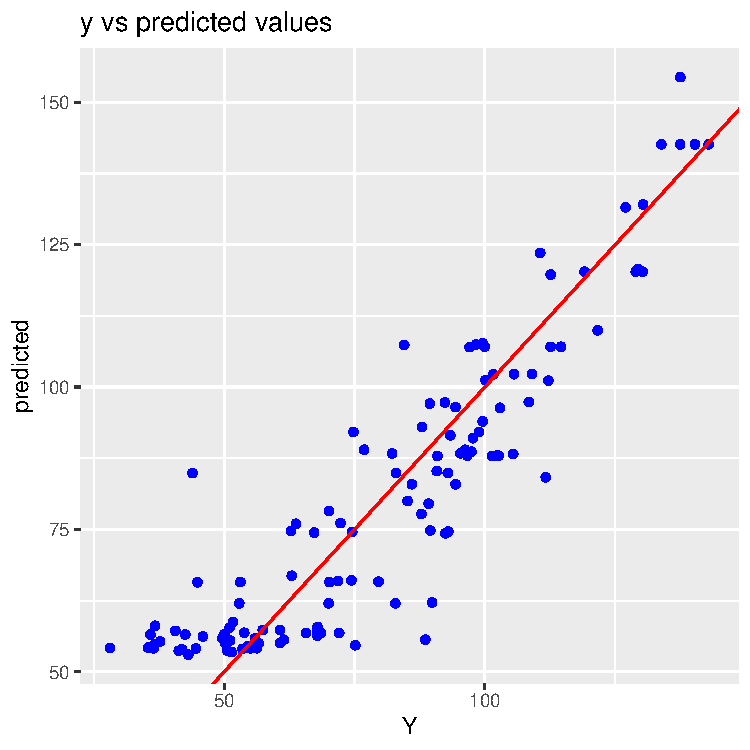
\includegraphics[width=0.5\linewidth]{figures/mlr/y_vs_predicted_values_full_model.pdf}
    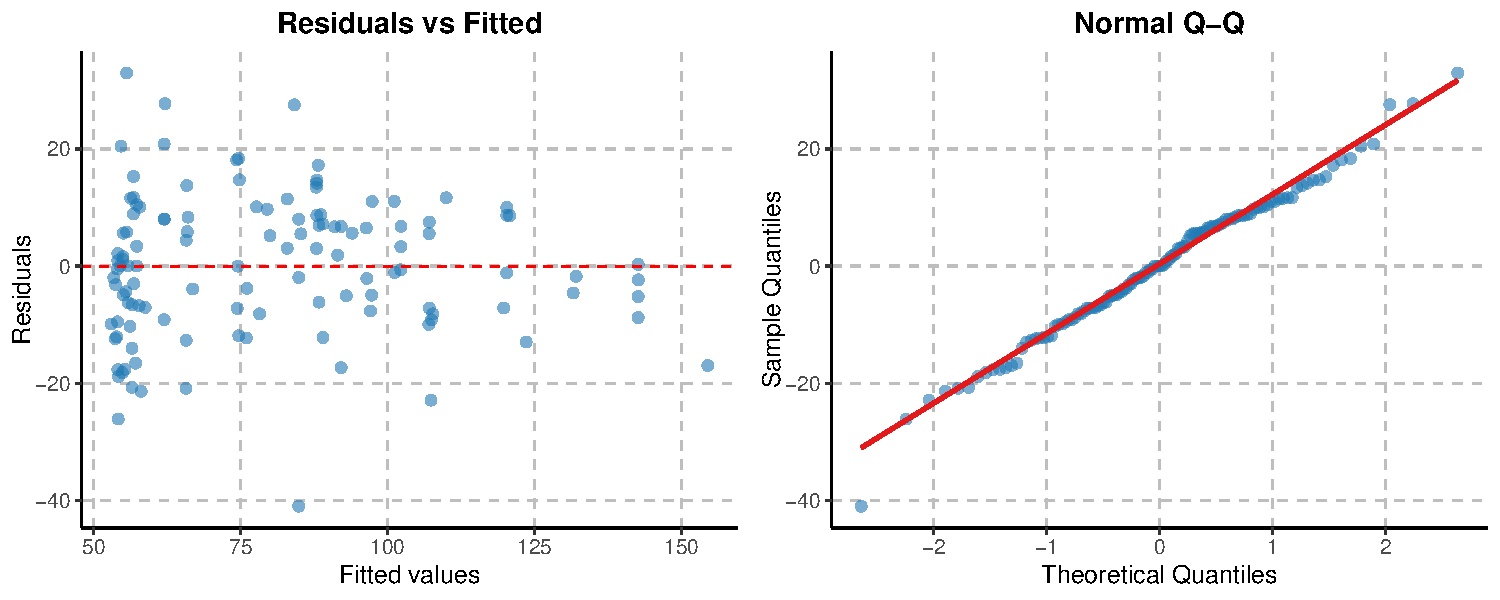
\includegraphics[width=1\linewidth]{figures/mlr/residuals_vs_fitted_qqplot.pdf}
    \caption{Regression model and residuals for the full model}
    \label{fig:full_mlr}
\end{figure}

\subsection{Adjusted Model}

Figure \ref{fig:full_mlr} shows the model prediction and residuals. We can find that the $\sigma$ of residuals are dependent with $y'$, so we need to adjust the transformation to make $\sigma$ a constant.

We succeed in the goal by doing the transformation
\begin{equation}\label{eq:trans_y_mlr}
y' = \log^4 y
\end{equation}

So the model becomes
\begin{equation}\label{eq:adjusted_model}
    \log^4 y = \beta_0 +\beta_1 \sqrt{x_1} + \beta_2 x_2 +\beta_3 x_3 + \beta_4 (2 - x_4) + \epsilon
\end{equation}

\begin{figure}
    \centering
    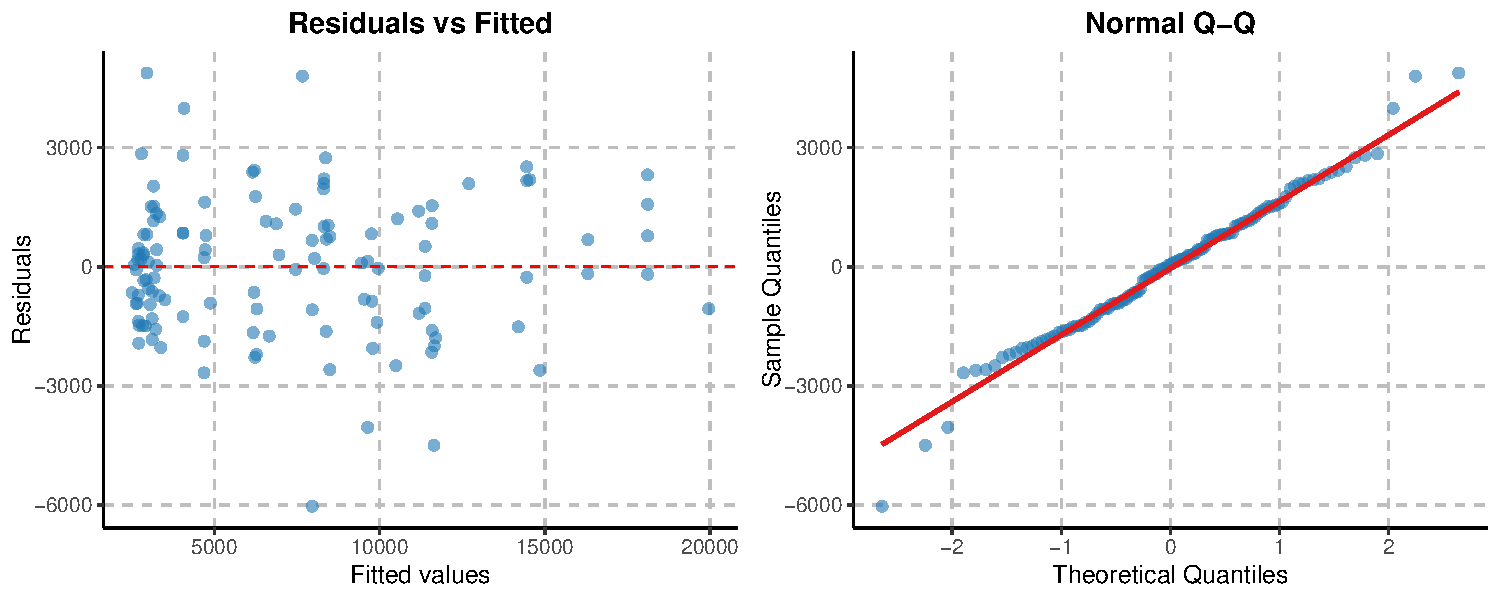
\includegraphics[width=1\linewidth]{figures/mlr/residuals_vs_fitted_qqplot_transformed.pdf}
    \caption{Regression model and residuals for the full model}
    \label{fig:adjust_mlr}
\end{figure}

Figure \ref{fig:adjust_mlr} shows residuals after adjustment. We can see that the $\sigma$ is mostly the same for each $y$.

\subsection{Adequacy Checking}

To check the adequacy of the model, we build an ANOVA / ANCOVA table for each variable. Shown in Table \ref{tab:mlr_anova}. We can find that $x_1', x_2, x_4'$ have information with $y$, while $x_3$ can be removed as it have a great $p$-value.

\begin{table}[ht]
    \centering
    \begin{tabular}{c|c|c|c|c}
    \toprule
        \textbf{Source} & \textbf{DF} & \textbf{RSS} & $\mathcal{F}$ & $p$-value \\
        \midrule
        Reduce $x_1$  & $117$ & $679542372$ & $99.815$ & $< 2.2\times 10^{-16}$\\
        Reduce $x_2$  & $117$ & $680342805$ & $100.07$ & $< 2.2\times 10^{-16}$\\
        Reduce $x_3$  & $117$ & $365429973$ & $0.0562$ & $0.8129$\\
        Reduce $x_4$  & $117$ & $459976649$ & $30.083$ & $2.457\times 10^{-7}$\\
        \midrule
        Full Model & $116$ & $365252858$ & & \\
    \bottomrule
    \end{tabular}
    \caption{ANOVA / ANCOVA table for adequacy checking.}
    \label{tab:mlr_anova}
\end{table}

So we decide to reduce $x_3$ from our model.

\subsection{Model Finalization}

So our final multiple linear regression model is 
\begin{equation}\label{eq:final_mlr}
    \log^4 y = \beta_0 +\beta_1 \sqrt{x_1} + \beta_2 x_2 +\beta_4 (2 - x_4) + \epsilon
\end{equation}

Figure \ref{fig:final_model} shows the predictions and residuals for the finalised model. We can observed that most of the residuals lie in the range $(-3000, 3000)$.

\begin{figure}
    \centering
    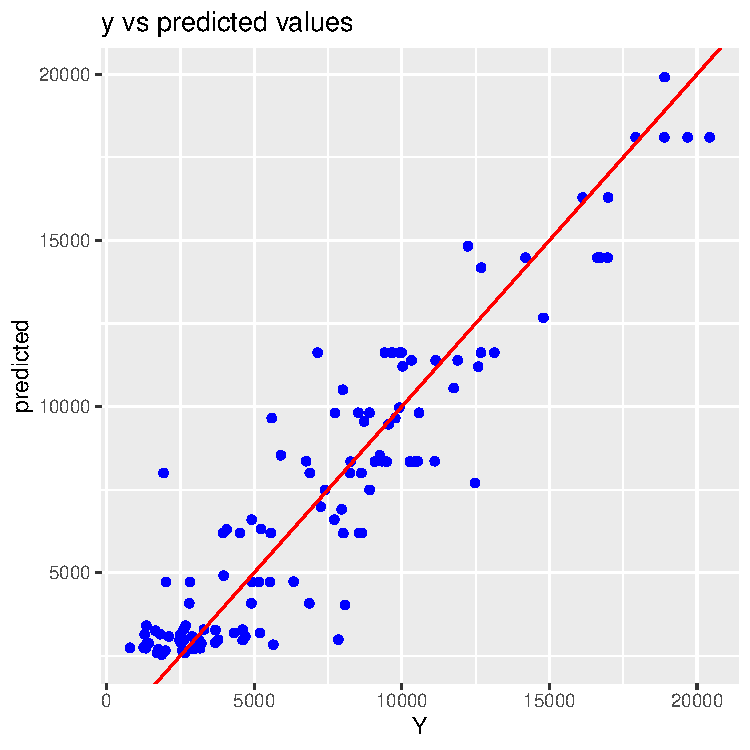
\includegraphics[width=0.5\linewidth]{figures/mlr/y_vs_predicted_values_reduced_model.pdf}
    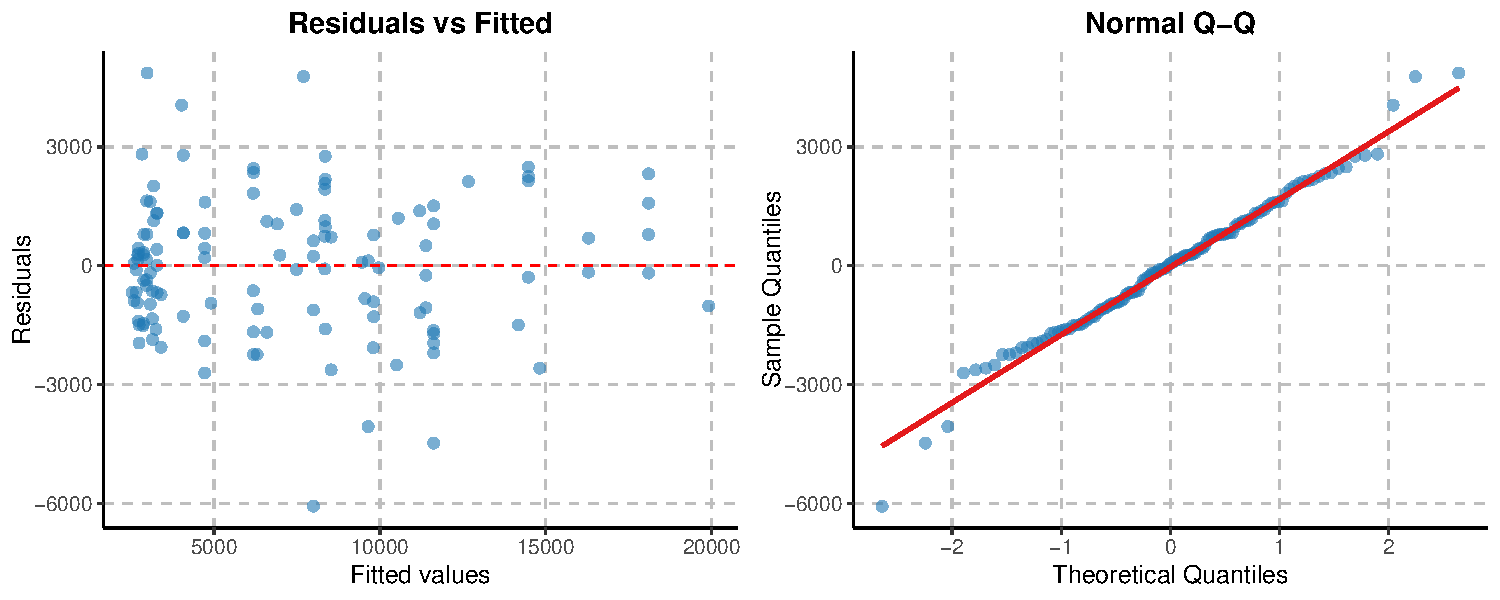
\includegraphics[width=1\linewidth]{figures/mlr/reduced_residuals_vs_fitted_qqplot.pdf}
    \caption{Predictions and residuals for the finalised model}
    \label{fig:final_model}
\end{figure}
